\section{Design}\label{sec:design_caida}

Fortunately, such projects exist. Two organizations, \caida and \ripe, maintain projects that do almost exactly that. \caida and \ripe (the latter through its "Atlas" project) have networks of thousands of small devices, typically Raspberry Pis or similar, that scan vast swathes of the internet, constantly running traceroutes (see \cref{sec:background_traceroutes}). For example, \caida's project involves a technique they call "prefix probing" where their network tries to run a traceroute to at least one device in every /24 prefix. Together these networks have generated terabytes of data over many years, all of which is publicly available.\footnote{\CAIDA's prefix probing data can be found at \url{https://www.caida.org/data/active/ipv4_prefix_probing_dataset.xml}. The \ripe Atlas data set may be found at \url{https://data-store.ripe.net/datasets/atlas-daily-dumps}}

\subsection{Direct Ping Calculation}

Since a traceroute is really just a series of pings, and a traceroute output reports the \rtts for all of them, \caida and \ripe Atlas traceroute data can be used for the everything-to-everything \rtt approach. The technique is simple: for every hop in each traceroute, record the source, the destination, and the \rtt. \IP address geolocation can be used to determine source and destination coordinates, and the haversine formula can be used to find a distance between them (\cref{form:haversine_distance}). This technique is referred to as \textit{direct ping calculation}.

\begin{formula}[h]
    \begin{equation}
        d = 2r\arcsin{\sqrt{\sin^2{\left(\frac{\rho_2-\rho_1}{2}\right)} + \cos{\rho_1}\cos{\rho_2}\sin^2{\left(\frac{\lambda_2-\lambda_1}{2}\right)}}}
    \end{equation}
    \caption{Haversine formula for distance; $\rho_1,\rho_2$ and $\lambda_1,\lambda_2$ are latitude/longitude respectively for the two points in radians, and $r$ is the radius of the Earth at 6,371 km.}
    \label{form:haversine_distance}
\end{formula}

\subsection{Indirect Ping Calculation}

\begin{figure}[h]
    \centering
    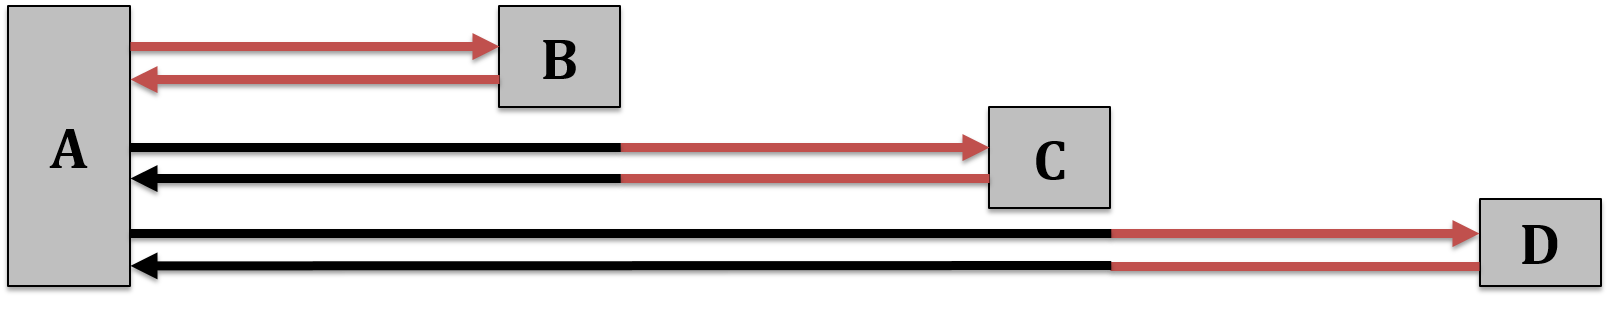
\includegraphics{caida/indirect_traceroute_diagram.png}
    \caption{Diagram of indirect traceroute ping calculation}
    \label{fig:indirect_ping_diagram}
\end{figure}

A crude calculation of the \rtt between each individual server in a traceroute can also be performed without directly sending pings between them. \Cref{fig:indirect_ping_diagram} shows roughly how this process works. Red lines indicate the time between servers that we \textit{want} to measure, while black lines indicate data that the server running the traceroute can actually give us. By subtracting a server's \rtt from the \rtt of the server just behind it, we can estimate the \rtt directly between the two. The same technique applies to any two arbitrary pairs of hops in the traceroute log, although a sanity check to guard against negative \rtts (caused by jitter along connections compounded by the subtraction operation) is needed.

This method results in almost double the amount of ping data per traceroute, since if you have a traceroute $A\rightarrow B\rightarrow C\rightarrow D$, you have data for not only $A\rightarrow B, A\rightarrow C,$ and $A\rightarrow D$, but you can also calculate $B\rightarrow C, B\rightarrow D$, and $C\rightarrow D$. More formally, for a traceroute of $n$ hops, you can extract $2n-2$ \rtts. This technique is referred to as \textit{indirect ping calculation}, and can similarly involve distance calculations provided by \cref{form:haversine_distance}.
